\subsection{Overview}
In order to design our application we need two main parts: one is the
The general architecture of our system has three tiers.
We have a mobile app running on mobile devices, smartphones or tablets with ios or Android.
then we have a server

the kind of architecture is distributed logic as explainde in the slides.


\subsection{Component view}

Here are proposed the component view for both part of the system, the mobile application and the application server.


\subsubsection{Mobile App}

The component view for the mobile app

\paragraph{Entities}
Entities are the domain of the system, they represent the business objects of the application. In our case entities are plain objects with methods that don't have any dependency on other part of the system (eg. frameworks).
Since the core of our system is based on \textbf{Users}, \textbf{Violations} and \textbf{Tickets} we have included those entities.
The last


\paragraph{Use Cases}
Use cases are here components that represent our system actions: it’s what is possible to do do with the application. We have one component for every possible use case.The use case doesn’t know who triggered it and how the results are going to be presented, but relies only

We encapsulate all use case in a \textbf{Use Case interactor} which manages all possible use cases and interacts with the entities.


\paragraph{Controller}


It's the job of the Controller to get fresh data from our Application  API, and the external i when there is an Internet connection (and then to cache it locally), or to get the cached data when the user is offline

\Controller

\begin{sidewaysfigure}[H]
\centering
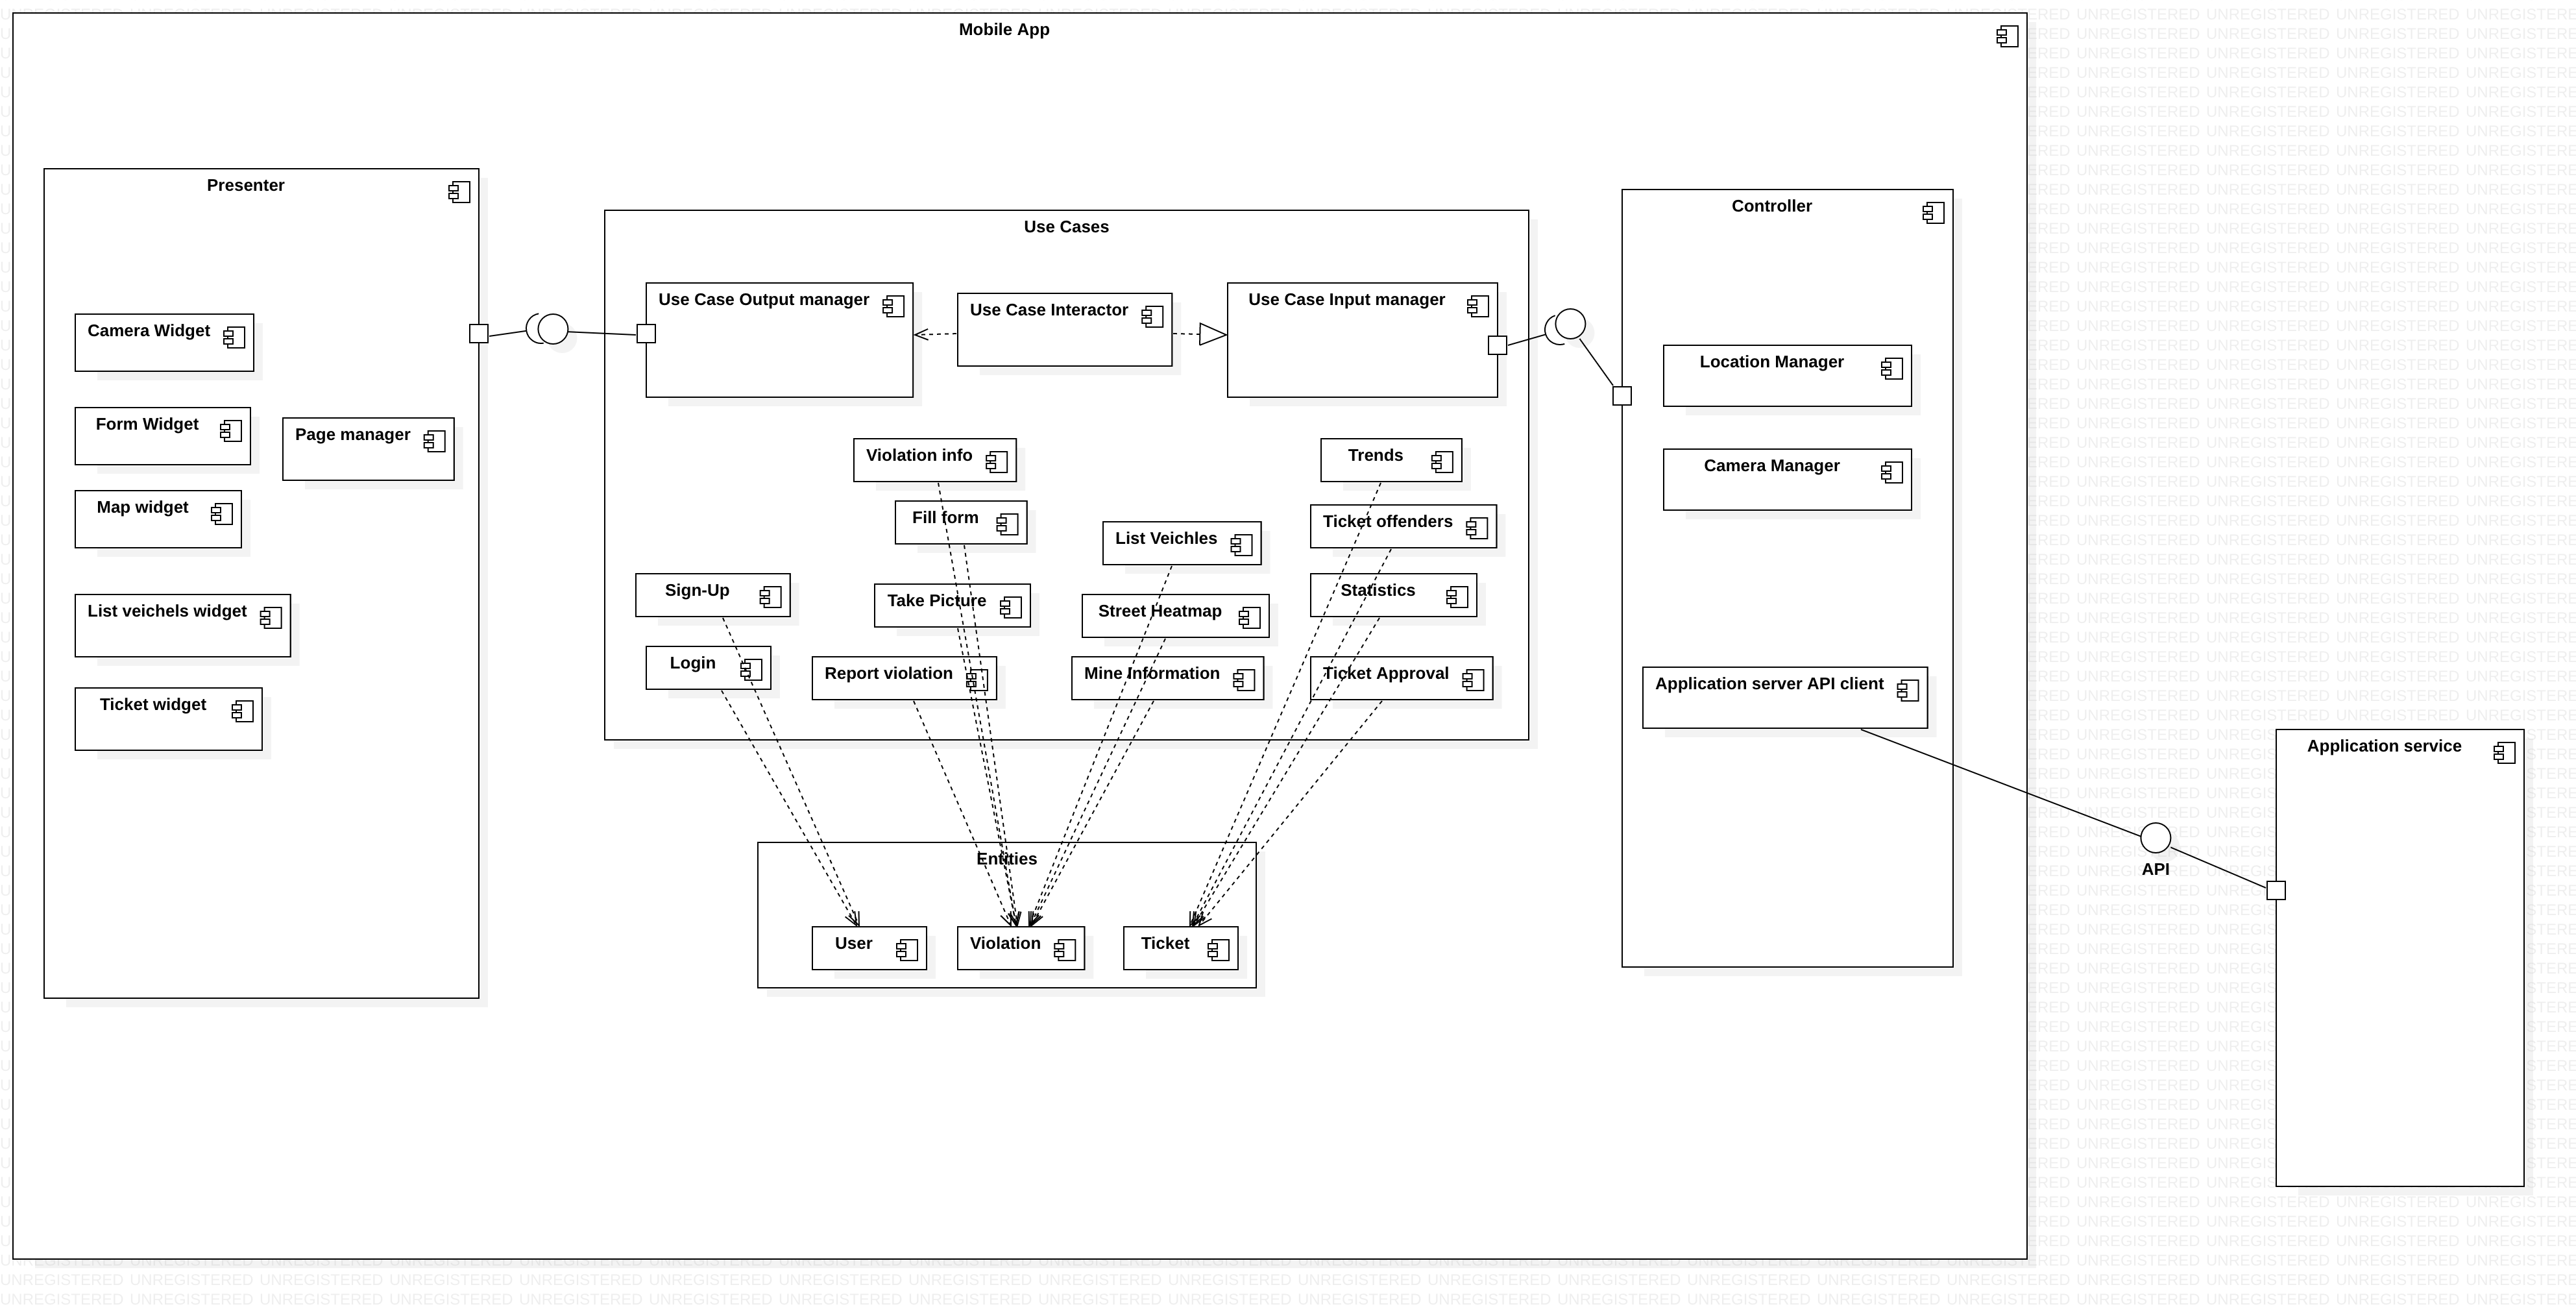
\includegraphics[width=\textwidth]{Images/ComponentDiagram1.png}
\caption{\label{fig:compdiag} Component diagram}
\end{sidewaysfigure}




\subsubsection{Application Server}

\begin{sidewaysfigure}[H]
\centering
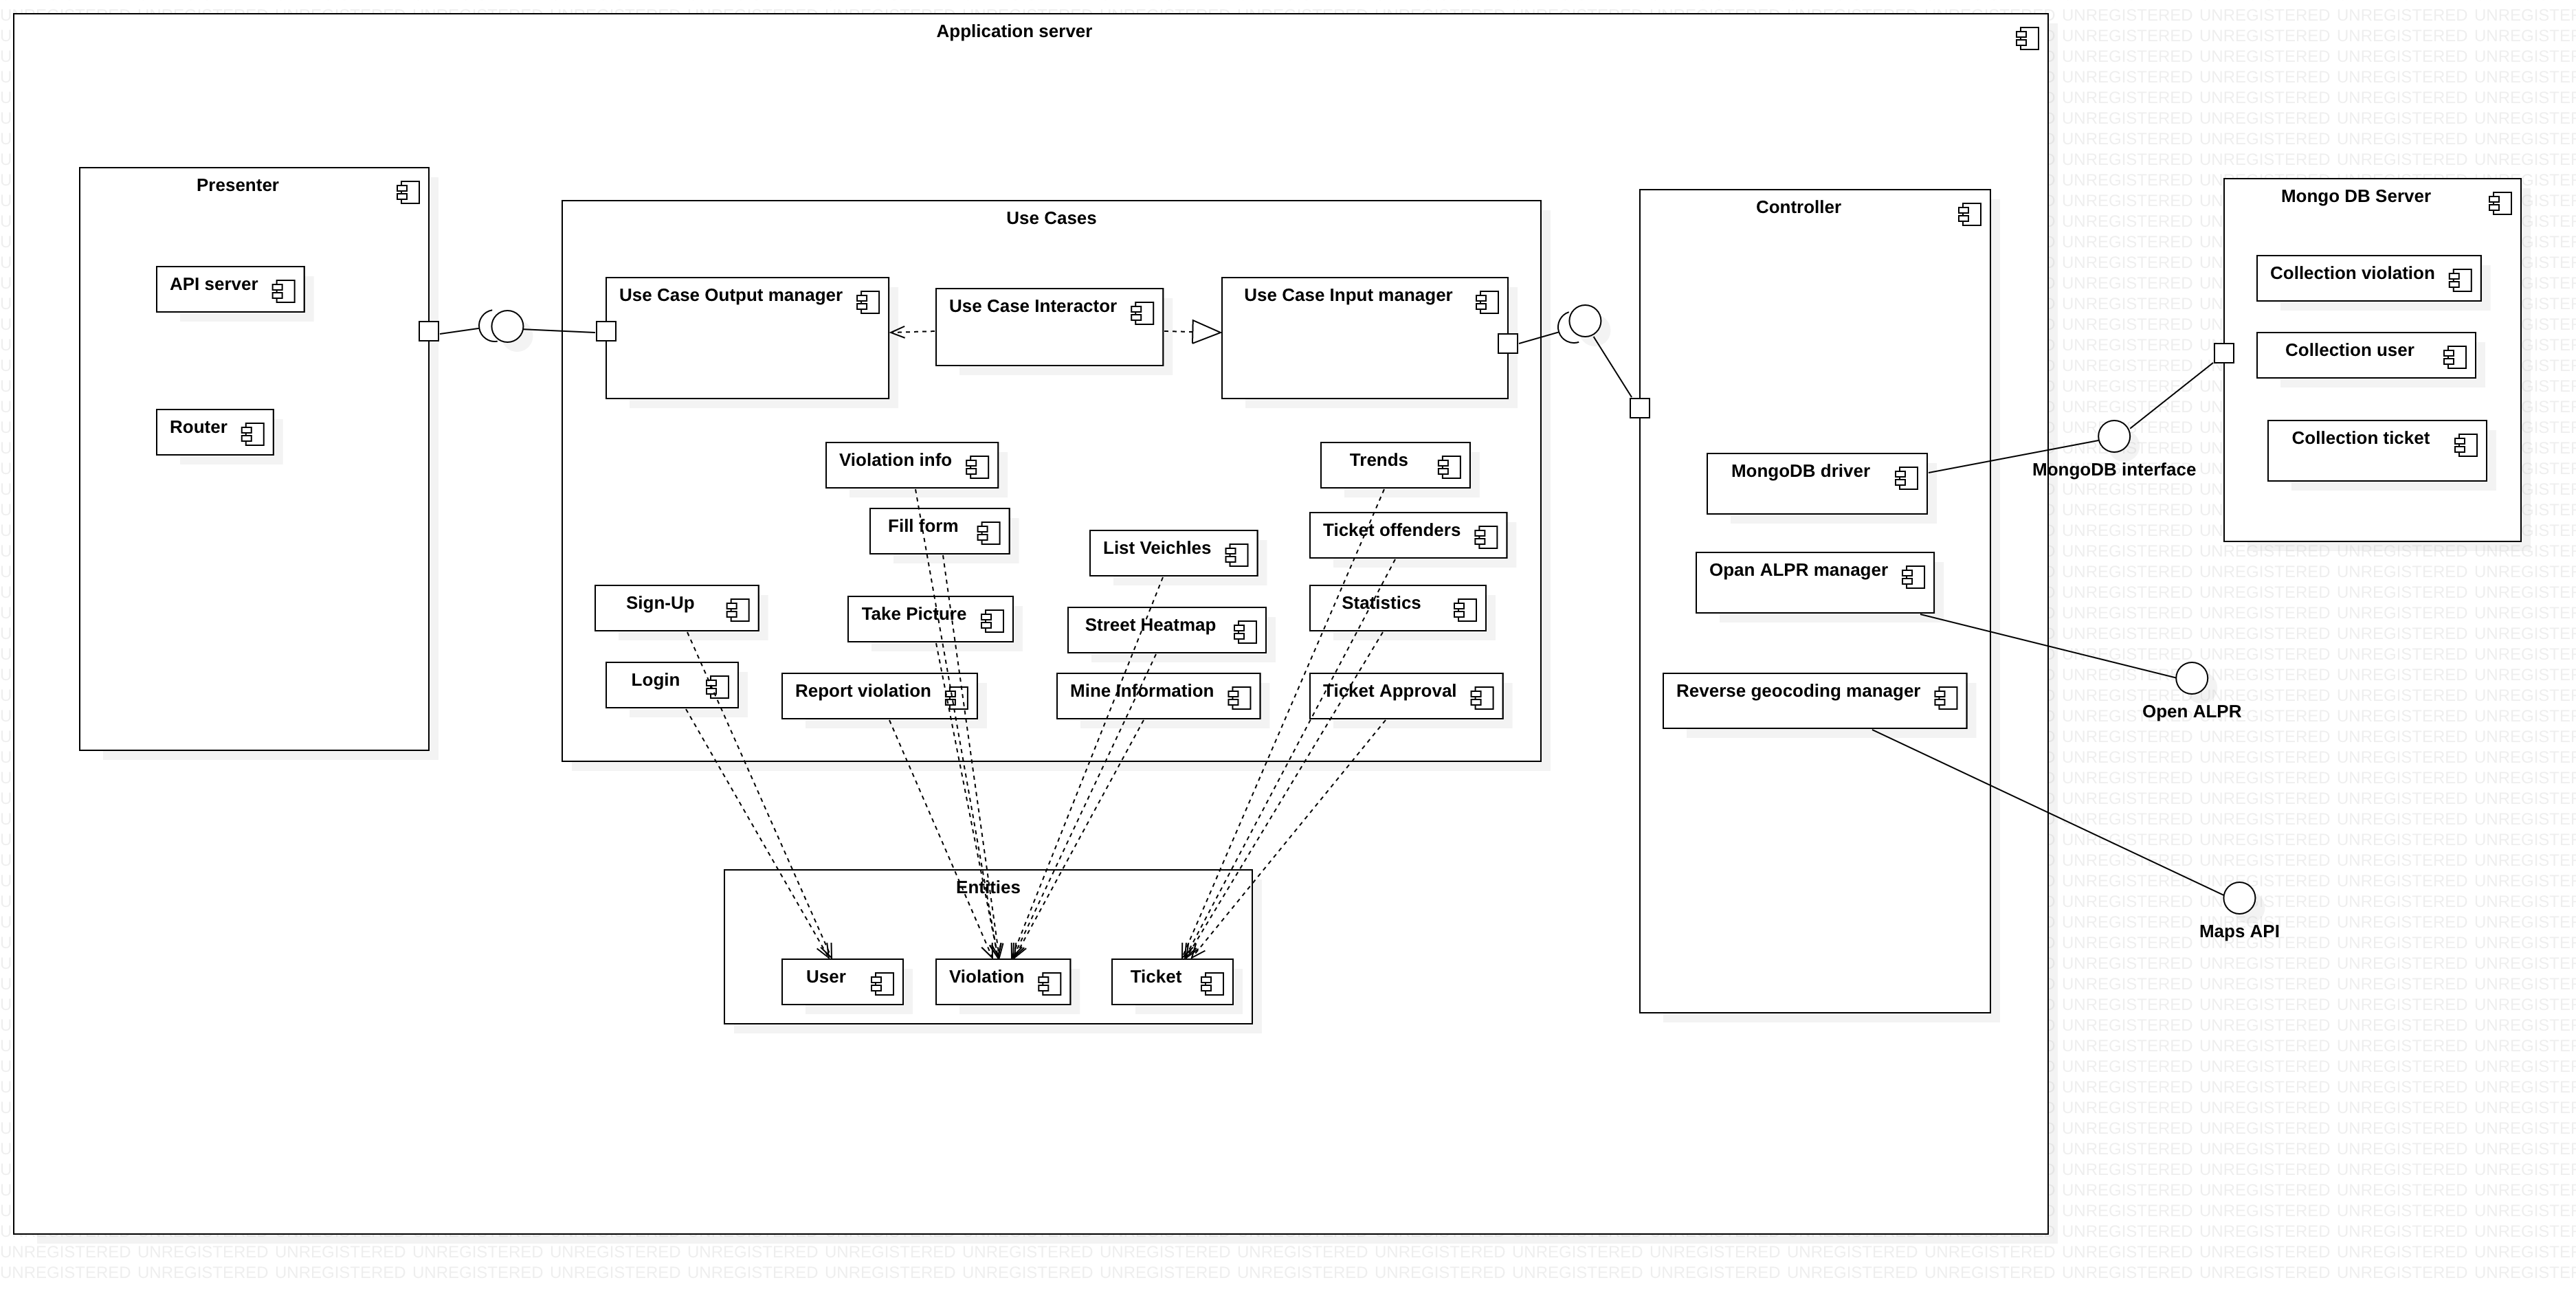
\includegraphics[width=\textwidth]{Images/ComponentDiagram2.png}
\caption{\label{fig:compdiag} Component diagram}
\end{sidewaysfigure}





\subsection{Deployment view}

In Figure \ref{fig:deploy} is shown the Deployment diagram.

The deployment consist of three main devices. The first tier consist is \textbf{Mobile device} the user will use, which can be a smartphone or a tablet using as operating system either iOS or Android.
The exection environment is the built Flutter app.


The second tier is the \textbf{Application Server}. It is supposed to be a dedicated server running a linux distribution specific for server use. As an example of OS we choose Centos 7. Other distros can be used like Red Hat Enterprise Linux, Debian, OpenSUSE.
As execution enviorment we install Node.js which is an open-source JavaScript runtime environment that executes JavaScript code outside of a browser. Inside Node.js we use the web application framework Express.js which is designed for building web applications and APIs.


The third tier is the \textbf{DB Server}. It consists in another server where we run the DB system MongoDB. We choose to run the database in a separate server and not in the same as the ApplicationServer in order to increase scalability. MongoDB is a cross-platform document-oriented database program. Classified as a NoSQL database program, MongoDB uses JSON-like documents with schema.



\begin{figure}
\centering
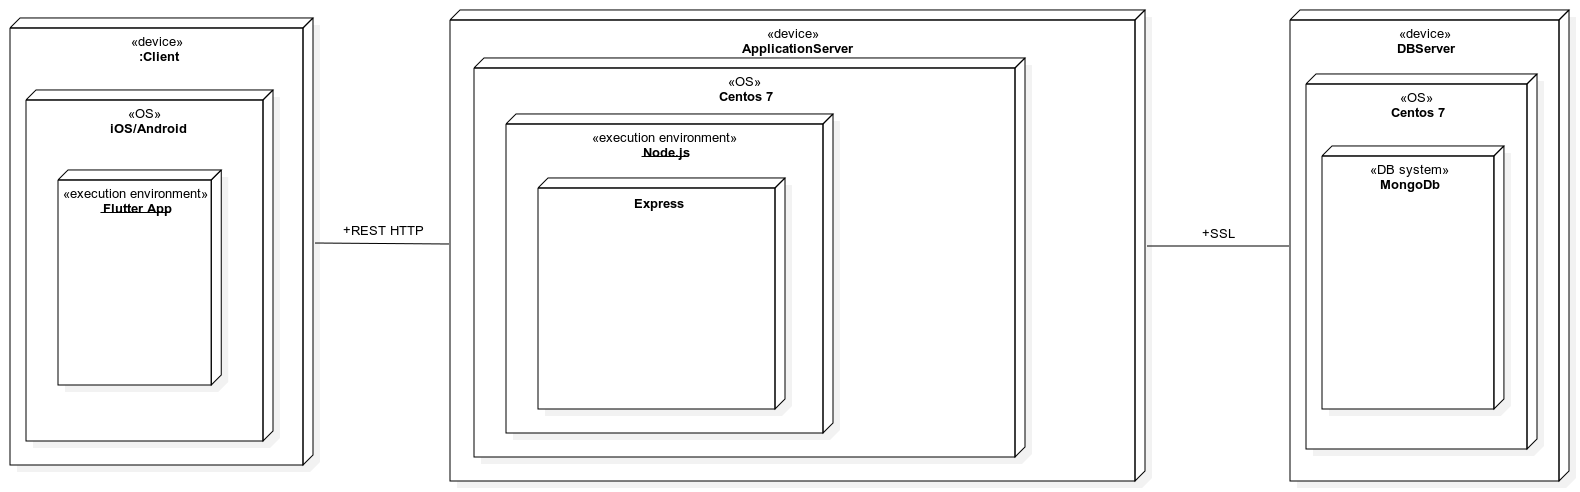
\includegraphics[width=\textwidth]{Images/DeploymentDiagram1.png}
\caption{\label{fig:deploy} Deployment diagram}
\end{figure}



\subsection{Runtime view}

\subsection{Selected Architectural styles and patterns}
This application will be developed with the MVP architectural pattern. In general, the MVP pattern allows separating the presentation layer from the logic, and this feature can be useful when we test the app. MVP is a user interface architectural pattern, which eases automated unit testing and it helps with providing clean code. This pattern consists of three parts which are Model, View and Presenter. In this pattern, model does not communicate with the view directly, it is the Presenter’s responsibility to communicate with the Model and update the View. SafeStreet application will be developed with the MVP architectural pattern in place of the MVC (model, view and controller) because of the test advantage mentioned above and compared to MVVM the architecture does not fit to the project design. MVVM does not give us a relation 1-1 between Presentation and View. For that reason, during this project it is recommended to utilize the MVP architectural pattern. There are more architectural patterns that we considered and discarded, like “Client-server pattern” or “Layered pattern”, but as mentioned above the MVP architecture would be the best fit for the SafeStreet Application.

\begin{figure}
\centering
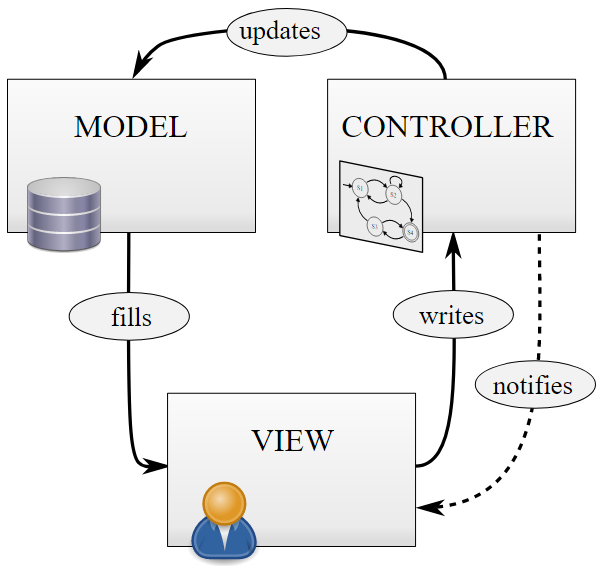
\includegraphics[width=\textwidth]{Images/MVC.png}
\caption{\label{fig:MVC} MVC Architectural diagram}
\end{figure}

\subsubsection{Model}
The model component stores data and its related logic. It represents data that is being transferred between controller components or any other related business logic. It responds to the request from the views and also responds to instructions from the controller to update itself. It is also the lowest level of the pattern which is responsible for maintaining data. In this project we use MongoDB database to store all the useful data. As well as we will use NODE.JS as the application server to build and run the application.

\subsubsection{View}
A View is that part of the application that represents the presentation of data.
Views are created by the data collected from the model data. A view requests the model to give information so that it resents the output presentation to the user.
In order to implement SafeStreet application we are going to use Flutter framework. Flutter helps app developers build cross-platform apps faster by using a single programming language. Although there are some other frameworks to implement cross-platform apps, according to [https://nevercode.io/blog/flutter-vs-react-native-a-developers-perspective/] Flutter is more efficient than others and has entered the cross-platform mobile development race very strongly.

\subsubsection{Controler}
Controler is the mediator between View and Model which hold responsibilities of everything which has to deal with presentation logic in the application. Presenter does the job of querying the Model, updating the View while responding to the user’s interactions. It monitors Model and talks to View so that they can handle when a particular View needs to be updated and when to not. In this project we will use Representational state transfer (REST) API in order to communicate between View and Model.REST is the software architectural style of the World Wide Web. REST gives a coordinated set of constraints to the design of components in a distributed hypermedia system that can lead to a higher-performing and more maintainable architecture.
To the extent that systems conform to the constraints of REST they can be called RESTful. RESTful systems typically, but not always, communicate over Hypertext Transfer Protocol (HTTP) with the same HTTP verbs (GET, POST, PUT, DELETE, etc.) which web browsers use to retrieve web pages and to send data to remote servers.
We have decided this API because it guarantees to achieve important non-functional requirements such as:
\begin{itemize}
 \item Scalability: every node belonging to our architecture can be multiplied without redesign the whole system.
 \item Portability: Every platform it's able to interact with the server since it's just a matter of HTTP request and JSON response.
 \item Reliability: If suddenly an instance crashes, the load balancer detaches it and will be replaced by a new one automatically.
\end{itemize}

\subsubsection{Why do we use MVP architectural pattern?}

Following are some reasons which makes MVP a good architectural pattern for our app:
\begin{itemize}
\item Makes debugging easier in Applications: MVP enforces three different layers of abstractions which makes it easier to debug your applications. Moreover, since business logic is completely decoupled from View, it is more easier to perform unit testing while developing your application.
\item Enforces better separation of Concerns: MVP does the great job of separating out the business logic and persistence logic out of the Activity and Fragment classes which in turn better enforce good separation of concerns.

\item Code Re-usability: In MVP, the code can be better reused since we can have multiple presenters controlling our Views. This is more important as we definitely don’t want to rely on a single presenter to control our different Views.
\end{itemize}


\subsection{Other design decisions}
